\chapter{Building damage}
\label{ch:damage}

\section{Introduction}
\label{sec:v-dam-intro}

This chapter describes the modelling of building damage. The
method is based on the HAZUS methodology \citep{dr_FEMA99b} with a
few modifications to suit the Monte-Carlo approach used in the
EQRM. The modifications are discussed at the end of this chapter.

The Capacity Spectrum Method\index{capacity spectrum method}
(\citealp{dr_FEMA99b}; \citealp{dr_Kircher97a}) is used to obtain
the peak building displacement and acceleration corresponding to
each earthquake. The peak displacement\index{peak displacement}
and acceleration are the dependent variables for fragility
curve\index{fragility curves}s \citep{dr_Kircher97a} which give
probabilities of being in certain damage states, for different
types of damage, structural (damage to main structure) and
drift-sensitive and acceleration-sensitive non-structural damage
(e.g. damage to non-structural internal walls).


%%%%%%%%%%%%%%%%%%%%%%%%%%%%%%%%%%%%%%%%%%%%%%%%%%%5
\section{The capacity spectrum method}
\label{sec:v-dam-capspect}

The capacity spectrum method\index{capacity spectrum method} is
used to find the peak displacement\index{peak displacement} and
peak acceleration\index{peak acceleration} for each
earthquake-building pair. To use this technique each building is
approximated by a single degree of freedom oscillator (SDOF)
\citep{dr_Chopra01c}.

A building's capacity (or response) to an incoming seismic wave,
is defined by the capacity curve\index{capacity curve}, a
monotonic increasing curve giving the $S_a$ as a function of the
spectral displacement\index{response spectral displacement} $S_d$.
The response spectral acceleration\index{response spectral
acceleration} ($S_a$) normally plotted against building period, is
plotted against spectral displacement\index{response spectral
displacement} $S_d$ (to describe the earthquake motion) in the capacity spectrum method. When
plotted this way the $S_a$ vs. $S_d$ plot is known as the demand
curve\index{demand curve}. The peak displacement\index{peak
displacement} and acceleration experienced by the building as a
result of the `induced motion' is modelled by the intersection of
the capacity curve\index{capacity curve} with the demand
curve\index{demand curve} (\fref{fig:vdamage-capspect}).

The response spectral acceleration\index{response spectral
acceleration} curve is normally defined by the attenuation model
with $5\%$ damping.  The actual damping generated by a building
differs from $5\%$ and is a function of the building attributes
such as structural type (see Section \ref{sec:grids-constructionclass}). The capacity
spectrum method\index{capacity spectrum method} allows for this
variation by adjusting the damping (see
\sref{subsec:v-dam-damping}).

\begin{figure}[htp]
\centering \psfrag{point}{$(S_d^*, S_a^*)$}
\psfrag{buildingcap}{capacity curve} \psfrag{response}{demand
curve}
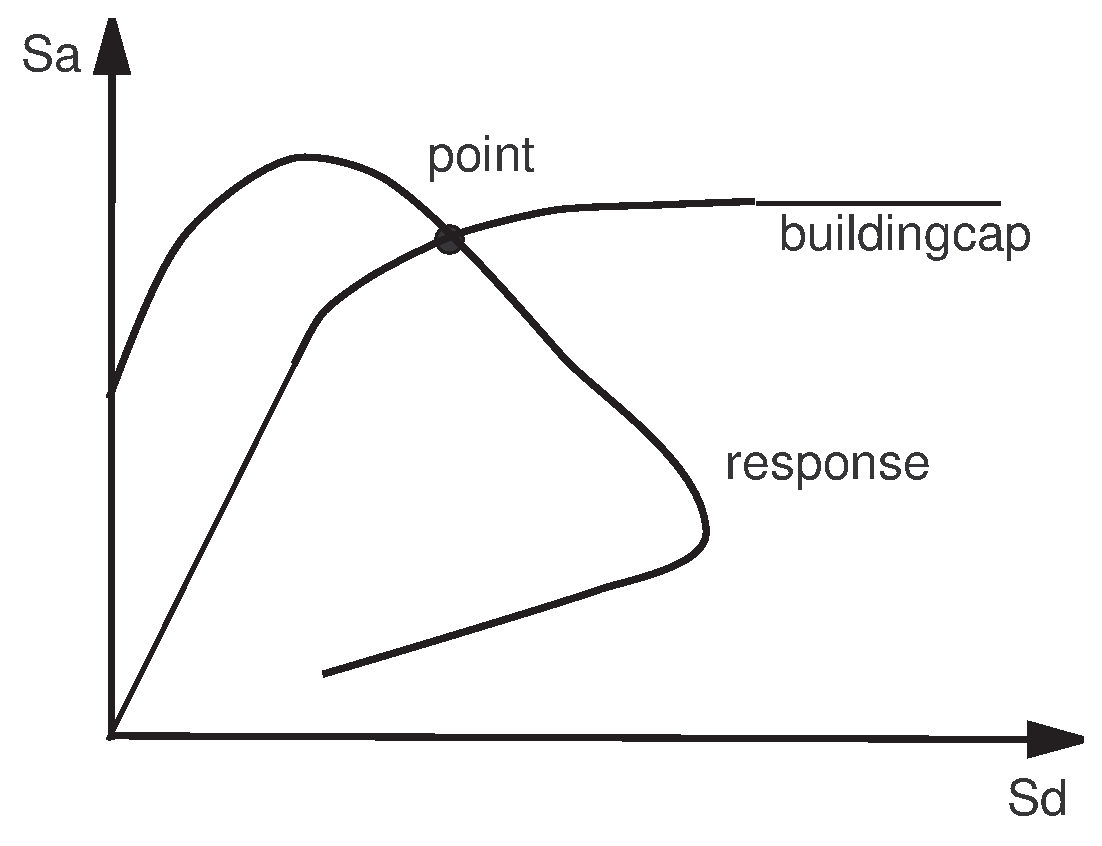
\includegraphics[height=0.3\textheight]{fig-vdamage-capspect}
\caption{The capacity spectrum method\index{capacity spectrum
method}.} \label{fig:vdamage-capspect}
\end{figure}


\fref{fig:vdamage-capspect} illustrates the intersection of the
capacity curve\index{capacity curve} with the demand
curve\index{demand curve}.  In the elastic region (or linear
component) of the capacity curve\index{capacity curve} the
intersection between the capacity curve\index{capacity curve} and
the appropriately damped demand curve\index{demand curve} occurs
at a period corresponding to the natural period of the building.
If the intersection occurs in the nonlinear plastic deformation
region, hysteretic damping results in a larger component of the
earthquakes energy being absorbed through damping in the building.
In an equivalent linear approach, this effectively reduces the
natural period of the building.


\subsection{The building capacity curve\index{capacity curve}}

The building capacity curve\index{capacity curve}\index{building
capacity curve\index{capacity curve}} is defined by two points:
the yield point $(D_y, A_y)$ and the ultimate point $(D_u, A_u)$.
For displacements below the yield point the building response is
elastic and the capacity curve\index{capacity curve} represented
by a straight line. For displacement amplitudes greater than the
yield point nonlinear effects such as plastic deformation cause
the rate of increase to reduce. The curve asymptotes towards the
ultimate point (see \fref{fig:vdamage-cap}).

\begin{figure}[htp]
\centering
\psfrag{yield}{$(D_y, A_y)$}
\psfrag{ult}{$(D_u, A_u)$}
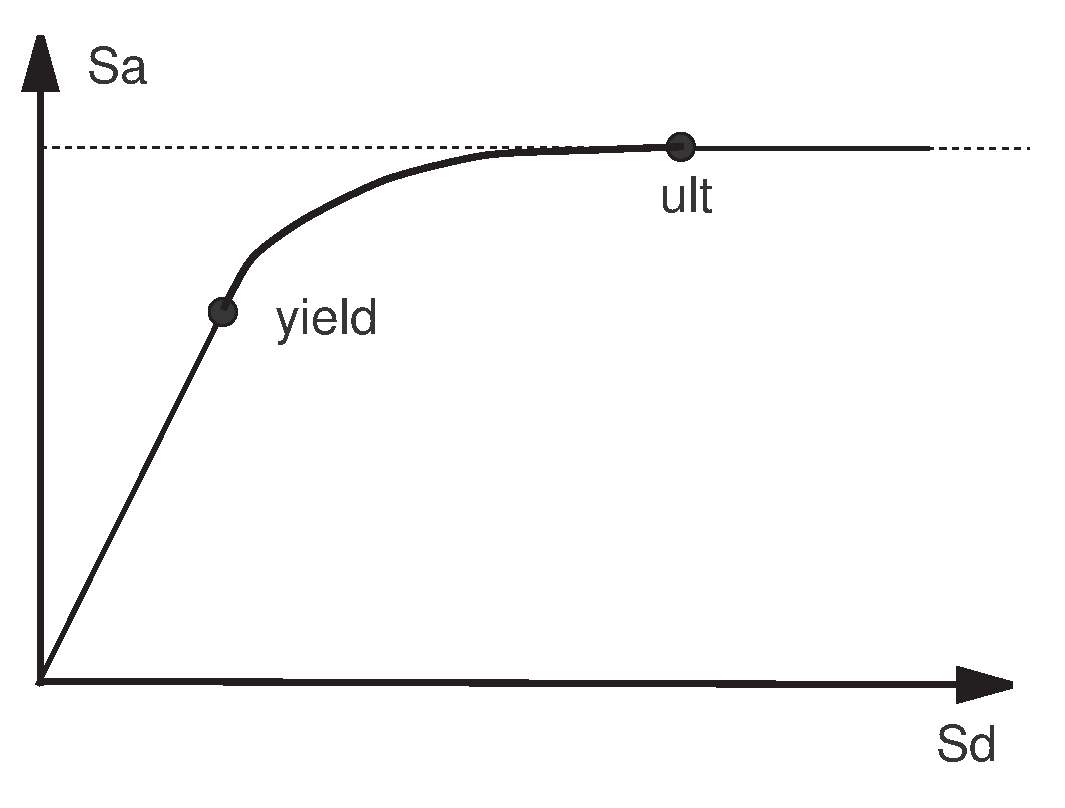
\includegraphics[height=0.3\textheight]{fig-vdamage-cap}
\caption{The graph of a typical building capacity
curve\index{capacity curve}, defined by
  the yield point $(D_y, A_y)$ and the ultimate point $(D_u, A_u)$.
  Note that the straight line between the yield point and the origin
  represents elastic behavior of the building. }
\label{fig:vdamage-cap}
\end{figure}


The yield point and ultimate point are defined in terms of the
building parameters as: $$ \begin{array}{rl}
 A_y = \frac{C_s\gamma}{\alpha_1} & [g],  \vspace{0.5em} \\
 D_y = \frac{1000}{4\pi^2}9.8A_y T_e^2 & [mm],\vspace{0.3em} \\
 A_u = \lambda A_y & [g], \vspace{0.3em} \\
 D_u = \lambda\mu D_y & [mm], \\
 \end{array}
$$
where the building parameters
\begin{align*}
C_s &= \text{design strength coefficient (fraction of the building weight)},\\
T_e &= \text{natural elastic building period (seconds)},\\
\alpha_1 &= \text{fraction of building weight participating in the
  first mode},\\
\alpha_2 &= \text{fraction of the effective building height to
building displacement},\\
\gamma &= \text{over-strength factor---yield to design strength ratio},\\
\lambda &= \text{over-strength factor---ultimate to yield strength ratio},\\
\mu &= \text{ductility factor},
\end{align*}
are given for several classes of building construction types
(\sref{sec:grids-constructionclass}). Note that the parameter
$\alpha_2$ is not used here, rather it is used to define the
appropriate damage ratios (see \eref{eq:damage-dstate}).


\subsubsection{Fitting the building capacity curve\index{capacity curve}}

The capacity curve\index{capacity curve} is composed of three
parts: a straight line to the yield point, a curved part from the
yield point to the ultimate point, and a horizontal line from the
ultimate point.


An exponential function is used to represent the curved part of
the building capacity curve\index{capacity curve}.  When defining
the curved section it is desirable that it has an identical slope
to the elastic part at the yield point and that its slope
approaches zeros at the ultimate point. We cannot satisfy all
these conditions with just three constants, however, we can
satisfy the condition of the curves matching at the ultimate point
approximately.

The form of the exponential curve is
$$
 y = c + a e^{-bx}
$$
where the constants $a$, $b$, and $c$ are given by
\begin{equation}
c = A_u,\quad b = \frac{k}{A_u-A_y}, \quad
a = (A_y-A_u)e^{b D_y}
\end{equation}
where $k = A_y/D_y$.

To obtain this, the following equation follows from the curves
joining at the ultimate points
$$
 c+ae^{-bD_u} = A_u.
$$
If we neglect the $e^{-bD_u}$ term, then $c=A_u$. From the
equation for the yield point we then obtain $A_u-A_y =
-ae^{-bD_y}$. From the equation that the slopes match at the yield
point we obtain $k = -abe^{-bD_y}$, where $k=A_y/D_y$ is the slope
of the elastic linear part of the capacity curve\index{capacity
curve}. Eliminating the exponential term from both these equations
gives the value of $b$, and the expression for $a$ follows. The
condition that the slope is zero at the ultimate point is
consistent with the assumption of neglecting the term $e^{-bD_u}$.
This will be true provided
$$
 \frac{D_u/D_y}{A_u/A_y-1} \gg 1.
$$
which will be generally true when the ultimate point is far from the
yield point.


\subsubsection{Variability of the capacity curve\index{capacity curve}s}
\label{sec:dam-capacity-var}

The uncertainty of the peak response of the building to a given
ground-shaking is incorporated by using a log-normal distribution
of building capacity curve\index{capacity curve}s with a
log-normal standard deviation parameter $\beta=0.3$. This value is
taken from \cite{dr_FEMA99b} for pre-code buildings whilst a value
of 0.25 is recommended for buildings constructed in alignment with
building codes. HAZUS gives no explanation or reference to how
these values were obtained. It was recommended in the Engineers'
workshop, \cite{dr_Stehle01a}, that a value $\beta=0.4$ be used
for Australian buildings, but there was no justification given for
this, so a value of $\beta=0.3$ has been retained.

The variability of the building capacity curve\index{capacity
curve} is described by a log-normal distribution for the vertical
component of the ultimate point. That is, $A_u=\bar A_u\times
e^{\beta\phi}$, where $\bar A_u$ is the median value of $A_u$ and
$\phi$ is a random number selected from a standardised normal
distribution.This sampling is
analogous to the random sampling technique used elsewhere in the
EQRM (e.g. \sref{attn:uncert-randomchoice}) because the median
 of a log-normally distributed random variable (e.g.$\bar A_u$) is the
 same as the exponential of the mean of the log (e.g. $exp(\mu_{ln(A)})$).
 This is illustrated in
\fref{fig:vdamage-capcurve-random}. The yield point $(D_y, A_y)$
on the random capacity curve\index{capacity curve} is chosen from
the equations $D_u=\lambda\mu D_y$, with $D_u=\bar D_u$, and $D_y
= 9.8A_yT_e^2$.

\begin{figure}[htp]
\centering
\psfrag{median}{median}
\psfrag{p1b}{$+\beta$}
\psfrag{m1b}{$-\beta$}
\psfrag{Sa}{$S_a$}
\psfrag{Sd}{$S_d$}
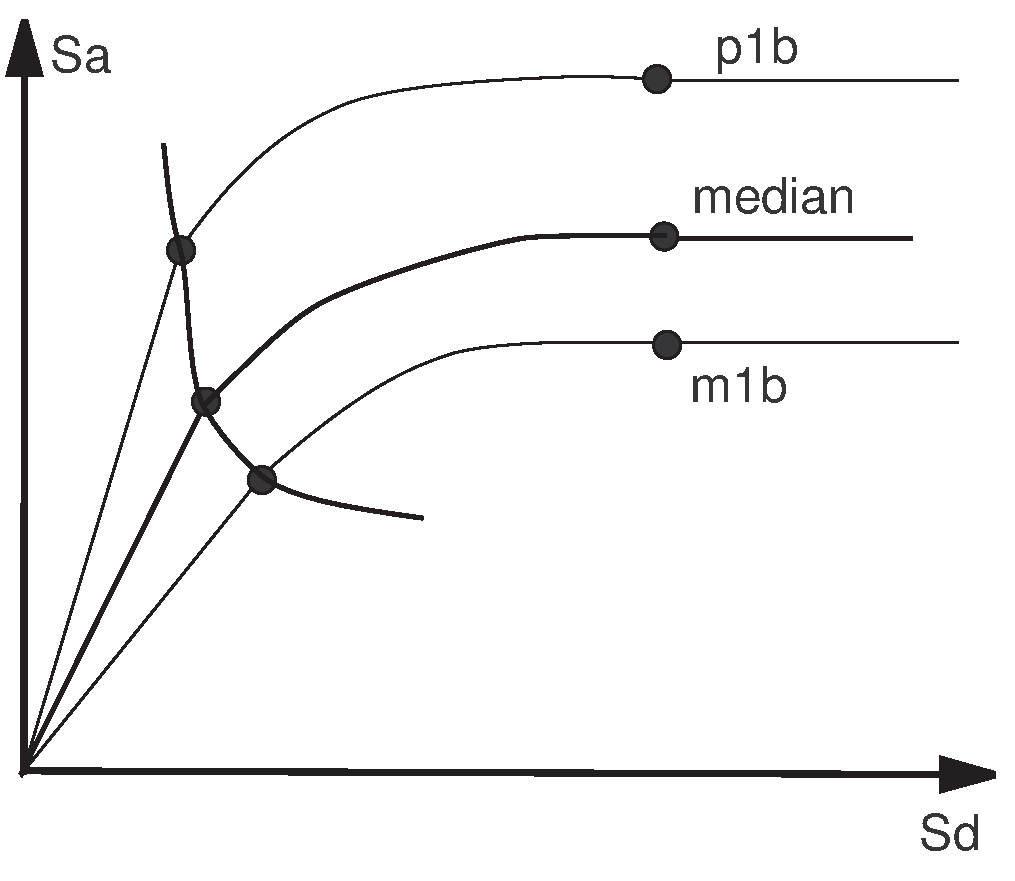
\includegraphics[width=0.6\textwidth]{fig-vdamage-caprand}
\caption{Illustration of the random selection of a building
capacity curve\index{capacity curve} from a log-normal
distribution of building capacity curve\index{capacity curve}s.
The median, 84th percentile ($+\beta$) and 16th percentile
($-\beta$) are shown.} \label{fig:vdamage-capcurve-random}
\end{figure}




\subsection{Damping the demand curve\index{demand curve}}
\label{subsec:v-dam-damping}

The Response Spectral Acceleration curve ($S_a$), as obtained from
an attenuation formula, is specified for 5\%\ damping. Recall that
$S_a$ describes the response of an idealised (SDOF) building. The
response of the actual building is incorporated by modifying the
damping. This is undertaken in the following two parts:
\begin{enumerate}
\item modification of elastic damping, and \item hysteretic
damping.
\end{enumerate}


\subsubsection{Modification of elastic damping}
\label{sec:damage-elasticdamping}

The HAZUS approach uses 5\%\ damping for all buildings. However,
the modifications suggested at the Australian buildings workshop
\citep{dr_Stehle01a} suggest using elastic damping values higher
than 5\%\ with corresponding hysteretic damping coefficients made
smaller. The values of the elastic damping have been determined
from \cite{Newmark82}.

Damping formulae are the same as used in \cite{dr_FEMA99b}, which
are obtained from \cite{Newmark82}. These are empirically derived
formulae, as multiplicative factors, defined for three regimes
according to building period. The three regimes correspond to the
acceleration-sensitive, velocity-sensitive and
displacement-sensitive areas of the response spectrum, denoted
$R_a$, $R_v$ and $R_d$ respectively. The effect of elastic damping
on the demand curve is illustrated in
\fref{fig:v-dam-damping-adrs}.

\begin{figure}[htp]
\centering
\psfrag{Sa}{$S_a$}
\psfrag{Sd}{$S_d$}
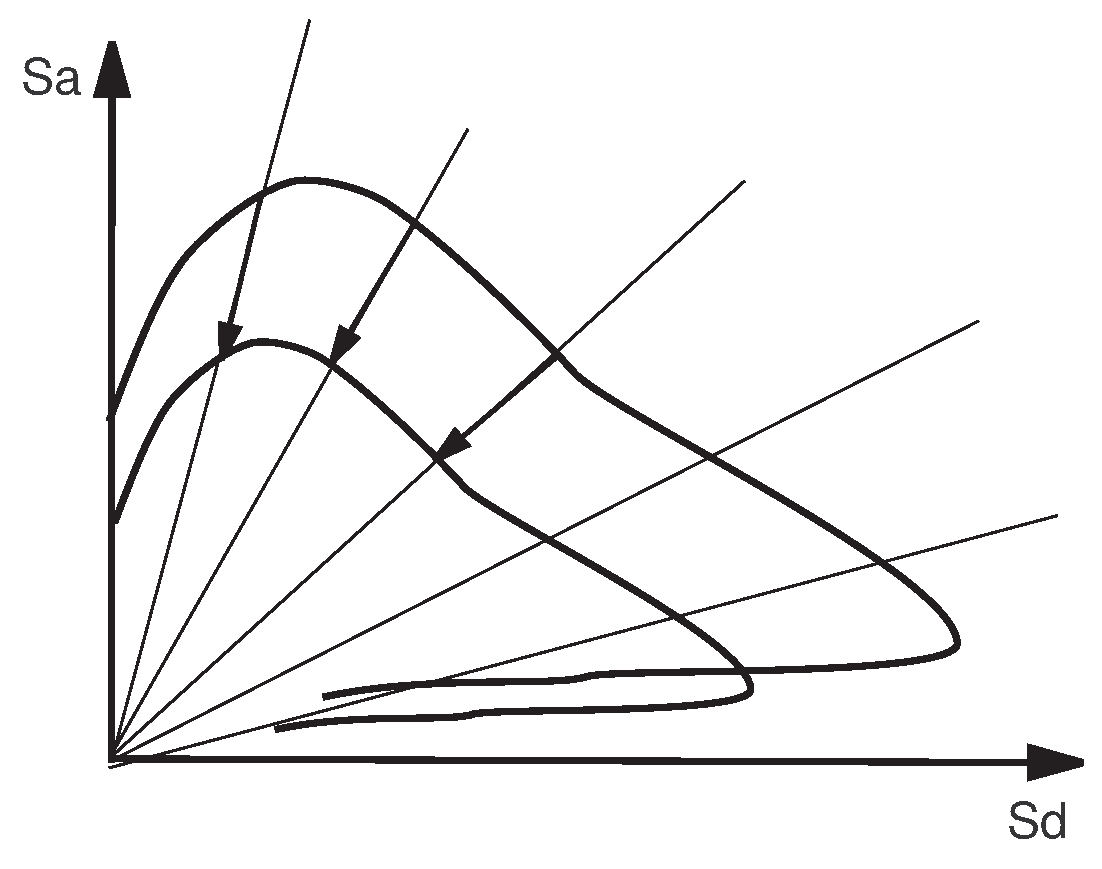
\includegraphics[width=0.5\textwidth]{fig-vdamage-damping}
\caption{Damping of the demand curve\index{demand curve}.}
\label{fig:v-dam-damping-adrs}
\end{figure}


The damping formula are:
\begin{align}
 R_a &= \frac{2.12}{3.21-0.68\ln(100\Beff)}, \quad 0\le T < T_{av}\\
\hspace{0.3em}
 R_v &= \frac{1.65}{2.31-0.41\ln(100\Beff)}, \quad T_{av}\le T < T_{vd}\\
\hspace{0.3em}
 R_d &= \frac{1.39}{1.82-0.27\ln(100\Beff)}, \quad T \ge T_{vd}
\end{align}
where $R_a$, $R_v$ and $R_d$ correspond to the
acceleration-sensitive, velocity-sensitive and
displacement-sensitive areas of the response spectrum and $\Beff$ is the effective damping\index{effective damping},
expressed as a decimal (not a percentage). Note that when $\Beff =
0.05$, (5\%\ damping) then $R_a=R_v=R_d=1$.

In the EQRM the user can set $R_d=R_v$, (HAZUS doesn't use $R_d$), or
$R_a$ and $R_d$ can be set to $R_v$. This might
be used if there are problems with convergence. The default
 uses all 3 factors.


The transition building periods (corner periods), $T_{av}$ and $T_{vd}$,
are given (according to HAZUS) as
\begin{equation}
 T_{av} = \frac{S_a(T_o =1.0)}{S_a(T_o =0.3)},
\qquad
 T_{vd} = 10^{(r_m-5)/2}
\end{equation}
where $r_m$ is the moment magnitude. These are called corner
periods because, in an `ideal' tripartite plot (i.e.~$S_v$ vs
building period, in log-log space), these periods correspond to
corners \citep{Newmark82}.

HAZUS also modifies $T_{av}$ to $T_{av\beta}$ where
$$
 T_{av\beta} = \frac{R_a}{R_v}T_{av}.
$$
It is not clear to the authors why this is needed. According to
discussions with Mark Edwards (\textit{pers. comm.}, 2002) it is
needed to account for the damping that has already occurred.
However, since the damping ratios are applied to the original
$5\%$ spectra, at each stage of the iteration, it should not be
needed.

Note that the formulae for the corner periods are chosen (by
HAZUS) to be consistent with the artificial standardised demand
curve\index{demand curve} that HAZUS uses. Therefore they are not
necessarily appropriate for response curves that are computed from
attenuation formulae. It is believed that they will be a
reasonable approximation. However, because our response spectra
are not consistent with the corner periods there may be some
problems with discontinuities leading to convergence problems with
the iterative approach used to deal with inelastic behavior (see
\sref{sec:dam-hystericdamping}). To try and minimise this a small
amount of smoothing of the demand curve\index{demand curve} is
applied near the corner periods.

For future work, it may be worth investigating using damping
formula which vary continuously as a function of period. Also, in
\cite{Newmark82} formula are given for a variability component of
the damping. A random damping factor has not yet been implemented.
It would not be difficult, but it first needs to be determined
whether it is already taken into account by the random capacity
curve\index{capacity curve}s.



\subsubsection{Hysteretic damping}
\label{sec:dam-hystericdamping}

When the intersection point occurs in the inelastic region the
damping applied to the response spectral
acceleration\index{response spectral acceleration} also has an
additional component due to hysteresis. This hysteretic damping
accounts for the fact that the buildings ability to absorb energy
changes after it has been pushed into the inelastic region. The
effective damping\index{effective damping} term $\Beff$ has an
elastic component $B_E$ and a component due to hysteretic damping
$B_H$ . This latter component is zero when the intersection point
is in the elastic region. The hysteretic damping term is
determined from the area enclosed by the hysteresis curve $A_H$,
as shown in \fref{fig:vdamage-hystarea}. The effective
damping\index{effective damping} is given by
\begin{equation}
\Beff = B_E + B_H,
\end{equation}
where
\begin{equation}
B_H = k \frac{A_H}{2\pi DA}
\end{equation}
and $B_E$ is defined by the process described in
\sref{sec:damage-elasticdamping}.
\begin{figure}
\centering
\psfrag{Sd}{$S_d$}
\psfrag{Sa}{$S_a$}
\psfrag{point}{$(S_d^*, S_a^*)$}
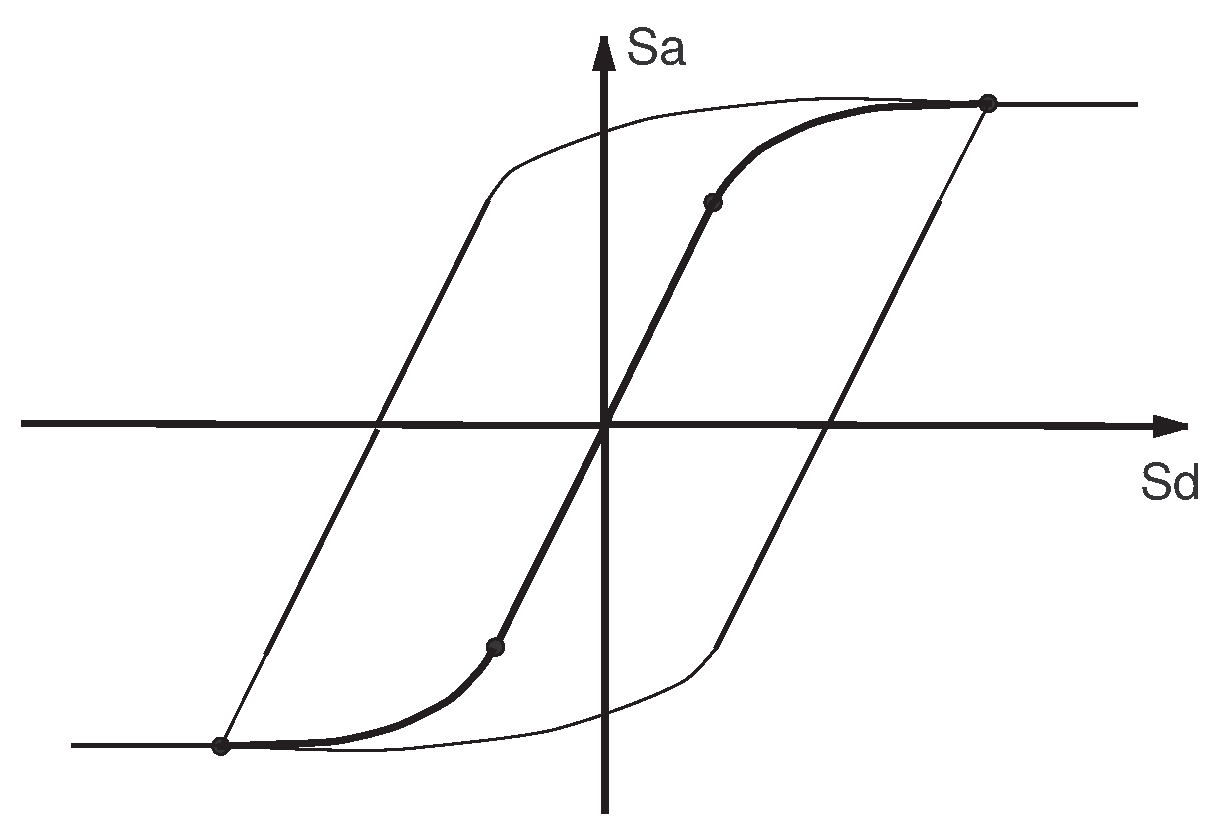
\includegraphics[width=0.4\textwidth]{fig-vdamage-hyst}
\caption{Hysteresis area.}
\label{fig:vdamage-hystarea}.
\end{figure}

Recall that the curved part of the hysteresis boundary is
approximated by
$$
 y = ae^{-bx}+c,
$$
where
$$
 c = A_u, \qquad
 b = \frac{k}{A_u-A_y}, \qquad
 a = (A_y-A_u)e^{b D_y}, \qquad
$$
and the slope of the elastic part is,
$$
 k = \frac{A_y}{D_y}.
$$

The area is calculated by subdividing into three separate areas
(see \fref{fig:vdamage-hyst3})
$$
 A_H = 2(A_1-A_2+A_3).
$$

\begin{figure}[htp]
\centering
\psfrag{A1}{$A_1$}
\psfrag{A2}{$A_2$}
\psfrag{A3}{$A_3$}
\psfrag{Sa}{$S_a$}
\psfrag{Sd}{$S_d$}
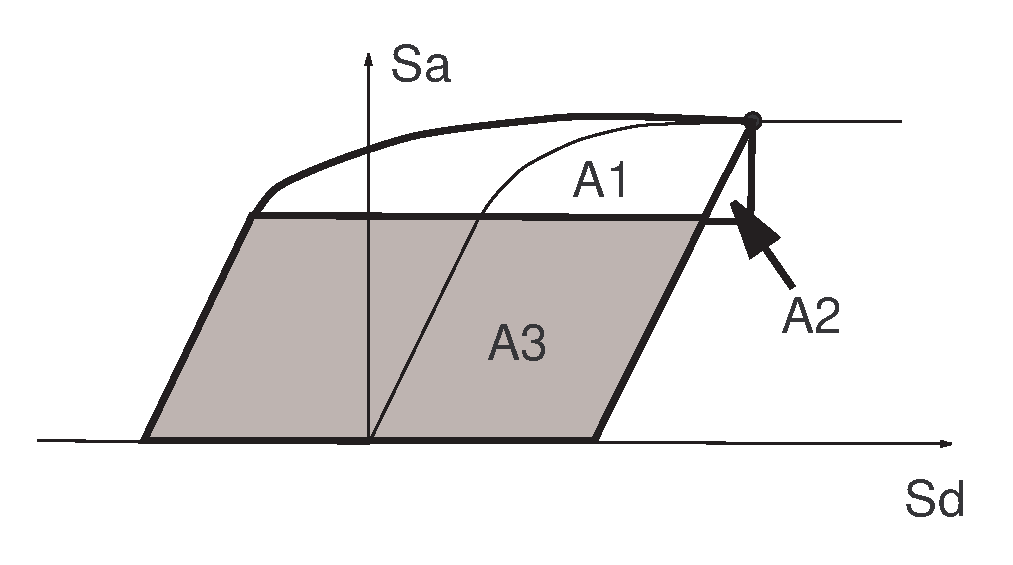
\includegraphics[height=0.3\textheight]{fig-vdamage-hyst3}
\caption{Diagram showing the sub-areas used for the hysteresis
area calculation.}
\label{fig:vdamage-hyst3}
\end{figure}


We also define the coordinates (see \fref{fig:vdamage-hyst2})
$$
x_2 = D-\frac{A}{k}, \qquad x_1 = 2x_2+\frac{y_1}{k}, \qquad y_1 =
A_u-A_y.
$$

\begin{figure}[htp]
\centering \psfrag{x1}{$x_1$} \psfrag{x2}{$x_2$} \psfrag{x3}{}
\psfrag{Sa}{$S_a$} \psfrag{Sd}{$S_d$} \psfrag{point}{$(D_u,A_u)$}
\psfrag{Ay}{$A_y$}
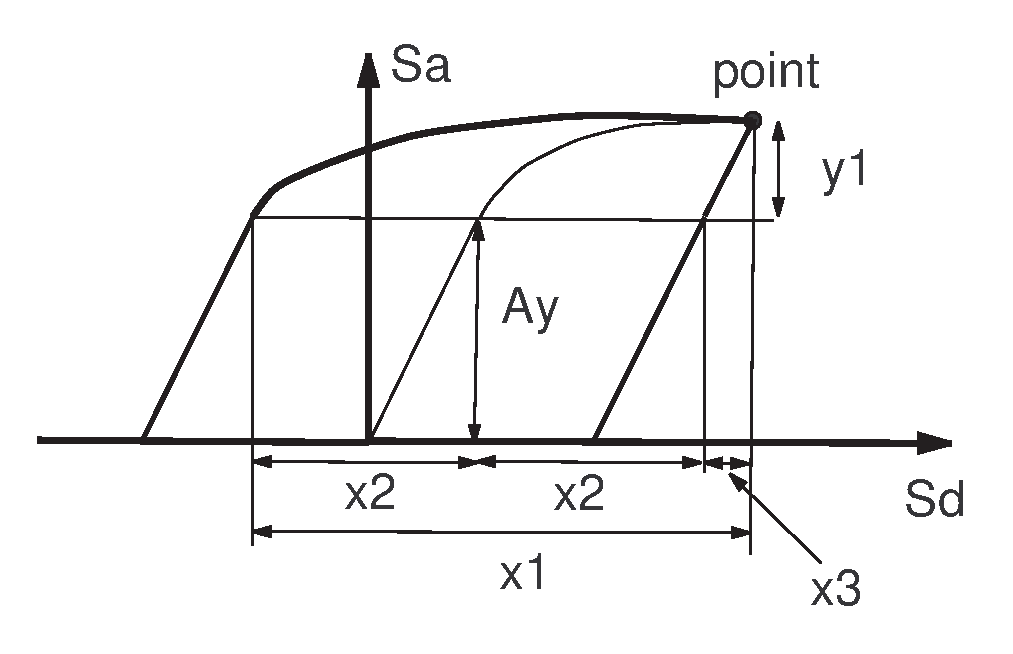
\includegraphics[height=0.3\textheight]{fig-vdamage-hyst2}
\caption{Coordinates used for hysteresis area calculation.}
\label{fig:vdamage-hyst2}
\end{figure}

The sub-areas are calculated as
\begin{align*}
 A_1 &= cx_1+\frac{a}{b}(1-e^{-bx_1})\\
 A_2 &= \frac{y_1^2}{2k}\\
 A_3 &= 2A_y(D-D_y).
\end{align*}

Currently the EQRM calculates
hysteretic damping for all events including those in the elastic
region (where the hysteretic damping is zero), because the
calculations are vectorised. Furthermore the code iterates until
the most nonlinear event has converged or the maximum iteration
limit is reached. Some efficiencies might be gained by first
filtering out those events in the elastic region, and then later
filtering out those events which have converged.


\subsection{Finding the intersection point}

The algorithm used to find the intersection point of the suitably
damped demand curve\index{demand curve} with the building capacity
curve\index{capacity curve} is quite simple. However, it is
vectorised over all the synthetic earthquakes. The intersection
point is generally not found exactly, rather it is approximated.

The algorithm can be summarised, as follows:
\begin{enumerate}
\item Locate points on demand curve\index{demand curve} and
building capacity curve\index{capacity curve} which bound the
intersection point, as shown in \fref{fig:vdamage-intersection}.
\item Use linear interpolation to find a first approximation to
the
  intersection point.
\item Use a vertical step to force the intersection to lie on the
  building capacity curve\index{capacity curve}.
\end{enumerate}


\begin{figure}[htp]
\centering
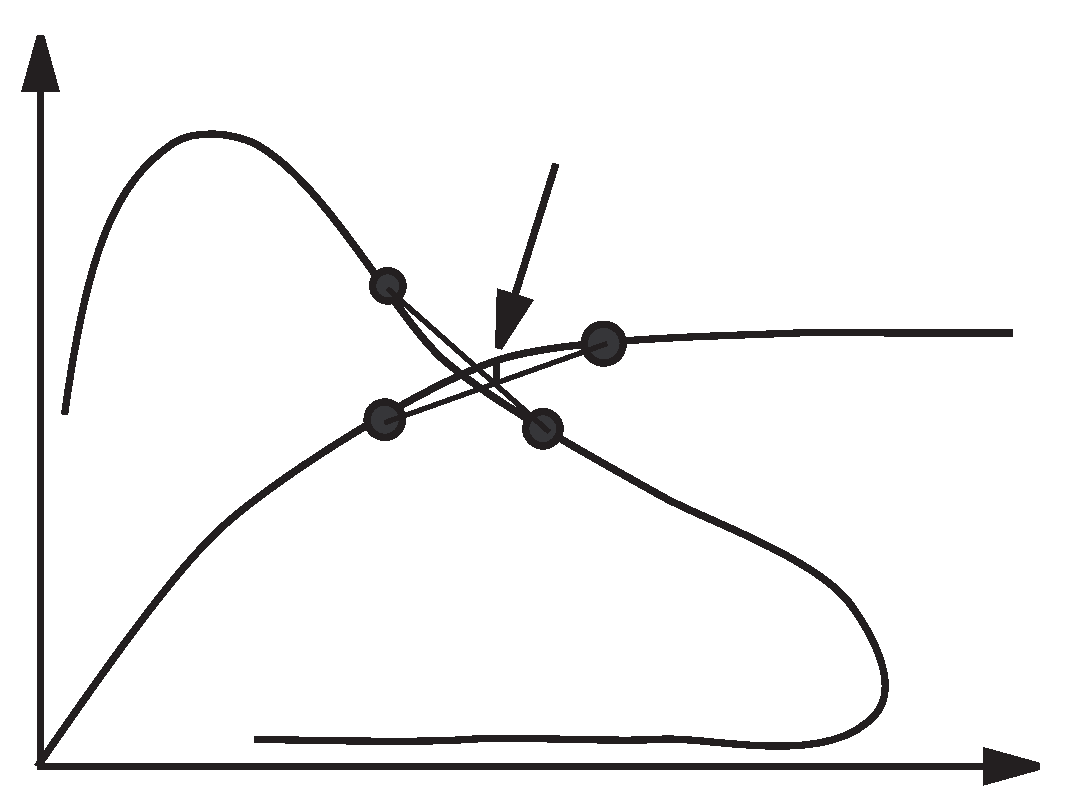
\includegraphics[height=0.3\textheight]{fig-vdamage-intersect}
\caption{Illustration of the algorithm used to approximate the
intersection point of the demand Sa curve and the building
capacity curve\index{capacity curve}.}
\label{fig:vdamage-intersection}
\end{figure}

It is important that the approximation to the intersection point
lies on the building capacity curve\index{capacity curve} for the
calculation of the hysteretic area.

Further refinements could be made to improve the accuracy of the
location of the intersection point. These might involve iterative
procedures which use the tangent of the capacity
curve\index{capacity curve} intersecting the line between the two
points on the demand curve\index{demand curve}, to iteratively
spiral into the true intersection point. However, a more
sophisticated scheme, such as this, may be difficult to code since
it would have to account for all possible variations in the form
of the demand curve\index{demand curve} (after soil amplification
and damping) and might not always converge. Therefore further
refinements are probably not warranted since the current scheme
appears to be sufficiently accurate.






%%%%%%%%%%%%%%%%%%%%%%%%%%%%%%%%%%%%%%%%%%%%%%%%%%%%%%%%%%%%%%%%%%%%%%%%%%%%%
\section{Fragility curves}

Fragility curves give the cumulative probability of a particular
building being in or exceeding a given damage state given  a
seismic demand parameter, such as building peak
displacement\index{peak displacement} or acceleration. There are
separate fragility curve\index{fragility curves}s for each of the
4 cumulative damage states: Slight, Moderate, Extensive and
Complete and the 3 types of damage: (a) Structural Damage (based
on peak displacement\index{peak displacement}), (b) Non-structural
damage-drift sensitive (also based on peak displacement\index{peak
displacement}) and (c) Non-structural damage-acceleration
sensitive (based on peak acceleration\index{peak acceleration}).

\citet[page 5-12, Table 5.2]{dr_FEMA99b} provides a table showing
typical non-structural components of buildings as drift sensitive
or acceleration sensitive. \citet[page 5-13 to 5-23]{dr_FEMA99b}
also provide qualitative descriptions of what the damage states
for structural and non-structural damage correspond to. For
example \textit{slight structural damage} for wood framed
construction corresponds to small cracks in door and window
openings and \textit{complete structural damage} corresponds to an
immediate danger of structure collapse.

In \citet[pages 5-19]{dr_FEMA99b} it is stated that non-structural
(acceleration sensitive) damage to components at or near ground
level may be better characterised by peak ground acceleration
(PGA) rather than peak spectral acceleration $S^*_a$. To this end,
HAZUS suggests a combined use of PGA and $S^*_a$ to model damage
for near ground components. Currently the EQRM considers only
$S^*_a$ when computing damage, however the HAZUS suggestion could
easily be incorporated into future version of the EQRM.


\subsection{Form of fragility curve\index{fragility curves}s}

Each fragility curve\index{fragility curves} is determined by two
parameters: the threshold value of displacement (or acceleration)
and a variability parameter. The form of the fragility
curve\index{fragility curves} is a cumulative log-normal
distribution,

\begin{equation}
\label{eq:vdamage-frag} 
P(damage \ge s_{dam} \Vert \bar S^*,S^*,\epsilon) =
[\Phi(\frac{ln(S^*) - ln(\bar S^*)}{\epsilon}]
\end{equation}


where $s_{dam}$ refers to the damage state of interest, $\Phi$ is
the standard cumulative normal distribution function,
$$
 \Phi(x) = \frac{1}{\sqrt{2\pi}}\int_{-\infty}^x e^{-t^2}\,dt,
$$
$S^*$ denotes either peak spectral displacement\index{response
spectral displacement}, $S_d^*$ or peak spectral acceleration,
$S_a^*$, $\bar S^*$ is the median damage state threshold value of
$S^*$ and $\epsilon$ is a variability parameter.

The value $\epsilon$ represents the uncertainty of the damage
state. It is the square root of the variance of the logarithm of
the data (i.e. the log-standard deviation). A zero value for
$\epsilon$ means the the curve approximates a step function, and
so below the threshold value the building is not in the given
damage state and above the threshold it is definitely in the
damage state. The larger the value of $\epsilon$ the more spread
out the curve is, reflecting our less certain knowledge of what
state the building is in (\fref{fig:dam-fragility-var-dstate}).


\begin{figure}[htp]
\label{fig:dam-fragility-var-dstate} \centering
\psfrag{Pr}{$F(s_{dam} \Vert \bar S^*,\epsilon)$}
\psfrag{Sd}{$S^*$} \psfrag{ST}{$\bar S^*$}
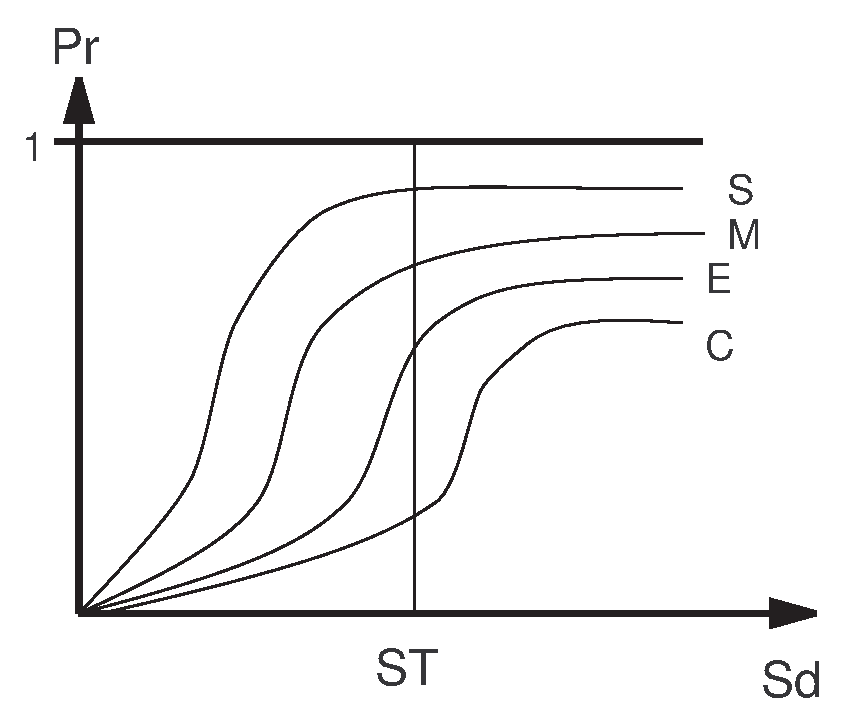
\includegraphics[height=0.3\textheight]{fig-vdamage-frag}
\caption{A typical fragility curve\index{fragility curves}, giving
the cumulative probability of
  being in or exceeding
  a certain damage state as a function of the
 peak displacement\index{peak displacement} (or acceleration).}
\label{fig:vdamage-frag}
\end{figure}

\subsection{Damage state thresholds}

The damage state thresholds are the median values that determine the
damage states.

For structural damage and non-structural drift-sensitive damage
the damage state thresholds are determined from provided drift
ratios for each building construction type. For non-structural
acceleration-sensitive damage the damage state thresholds are
obtained from specified acceleration thresholds. For example

\begin{equation}
\label{eq:damage-dstate}
 S_T = \alpha_2 h\delta
\end{equation}

is used to compute the median damage state threshold for
structural damage, where $\delta$ is the drift ratio, $h$ is the
provided height of the building for the given building
construction type and $\alpha_2$ is a building construction
parameter corresponding to the fraction of the building height
(roof) at the location of push-over mode displacement. The
parameters $\alpha_2$ and $h$ are given in Section
\ref{sec:grids-bdatabase}. Note that $h$ is given in
feet, however, in the code this is converted into $mm$ (since
$S_d$ is considered throughout the code in $mm$). Tables of drift
ratios, and acceleration values, for different sets of building
parameters are given in Section \ref{sec:grids-bdatabase}.


\subsection{Variability of the damage states}

The uncertainty of a building being in a given damage state for a
given peak displacement\index{peak displacement}, is characterised
by the variability parameter $\epsilon$ in equation
\eref{eq:vdamage-frag}. As this uncertainty becomes smaller, the
fragility curve\index{fragility curves} steepens and becomes more
like a step function, as shown in \fref{fig:vdamage-frag-var}.

\begin{figure}[htp]
\centering \psfrag{vert}{$F(s_{dam} \Vert \bar S^*,\epsilon)$}
\psfrag{hor}{$S^*$}
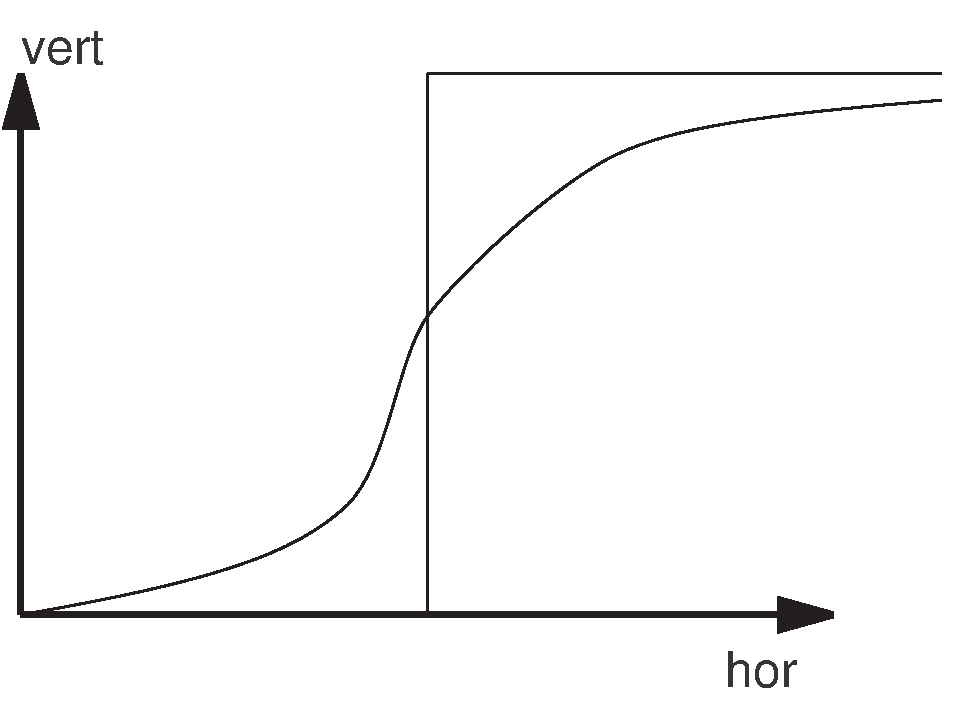
\includegraphics[height=0.3\textheight]{fig-vdamage-frag-step}
\caption{As the variability of a fragility curve\index{fragility
curves} is reduced the
  fragility curve\index{fragility curves} steepens and becomes more like a step function.}
\label{fig:vdamage-frag-var}
\end{figure}


We follow \cite{dr_FEMA99b} in setting
\begin{itemize}
\item for structural damage $\epsilon=0.4$, \item for
non-structural, drift sensitive damage $\epsilon=0.5$, \item for
non-structural, acceleration sensitive damage,
  $\epsilon=0.6$.
\end{itemize}
Note that HAZUS does not give any references to the derivation of
these values.


\subsection{Incremental probabilities}

The fragility curve\index{fragility curves}s give the probability
of being in the given damage state or a more destructive damage state. That is, they are
cumulative probabilities. For our Monte Carlo simulation approach
we need the incremental probabilities of the building being in the
given damage state. For example,  suppose we have the fragility
curve\index{fragility curves} for the extensive damage state,
$\Pr(d \le E)$. To find $\Pr(d=E)$, we calculate
$$
\Pr(d=E) = \Pr(d \ge E) - \Pr(d \ge C).
$$
This is illustrated in \fref{fig:vdamage-frag-inc}.

\begin{figure}[htp]
\centering
\psfrag{Sd}{$S^*$}
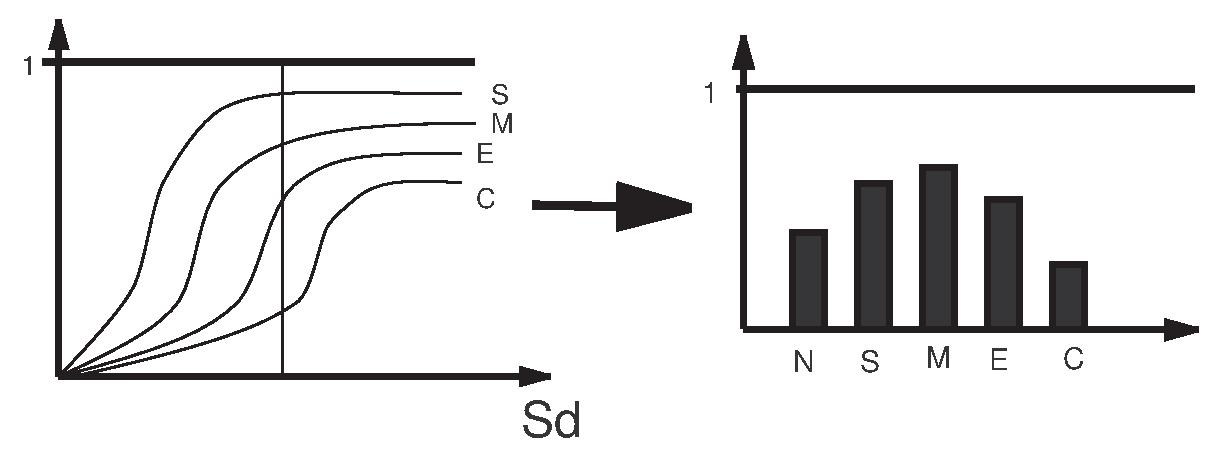
\includegraphics[width=0.95\textwidth]{fig-vdamage-frag-inc}
\caption{Converting the cumulative
  probabilities in the fragility curves\index{fragility curves} to incremental probabilities
  describing the probability that the building component is in a given damage state.}
\label{fig:vdamage-frag-inc}
\end{figure}


\section{Differences from HAZUS methodology}


A key difference in our implementation of the Capacity Spectrum
Method\index{capacity spectrum method} to that used by HAZUS is
using the full response spectrum for intersecting with the
building capacity curve\index{capacity curve} rather than a design
spectra based on only a few building periods. For example, the
HAZUS approach only uses periods 0.3 and 1.0 seconds. Our approach
has the advantage that the full structure of the response spectrum
and all the available information for the soils amplification
factors, at all periods, is taken into account rather than at only
two periods (\creftwo{ch:atten}{ch:reg}). There are also some
minor differences in the way that demand curve damping is applied.

Another difference is in how the fragility curve\index{fragility
curves}s are used. In HAZUS, the fragility curve\index{fragility
curves}s incorporate not only the variability of the damage state
thresholds, but also the variability of the capacity
curve\index{capacity curve} and the ground-shaking. A `convolution
procedure', as described in \cite{dr_Kircher97b}, is used to
convolve the various log-normal probability distributions for
ground-shaking and building capacity curve\index{capacity curve}
by calculating intersection points for a range of randomly
selected demand and capacity curve\index{capacity curve}s, then
fitting a log-normal distribution. In the EQRM the fragility
curve\index{fragility curves}s includes only the variability for
being in the given damage state and not the variability associated
with ground shaking or building type\index{building type}. The
variability associated with the fragility curve\index{fragility
curves} is defined by a cumulative log-normal distribution with
variability parameters $0.4$, $0.5$ and $0.6$ for structural
damage, non-structural damage (drift sensitive) and non-structural
damage (acceleration sensitive), respectively. The variability
associated with ground shaking
(\sreftwo{attn:uncertainty}{sec:regolith-incorp-unc}) and building
type (\sref{sec:dam-capacity-var}) are incorporated elsewhere in
the Monte-Carlo simulation.

\subsection{Extra features}

The risk component of the EQRM also has a number of extra features
or alternative operation modes that are not offered by the HAZUS
methodology. The most significant extra feature is:
\begin{enumerate}
\item The use of \textbf{uniform hazard spectra} instead of demand
curve\index{demand curve}s. This effectively drives the risk
calculation by hazard values rather than individual earthquakes.
The process is discussed further in \citet{dr_Patchett04a}. 
\end{enumerate}

